%25 Dec 2004
%O+I+Daniel+ dominic => final

\ifx\wholebook\relax\else
\input{../Common.tex}
\input{../macroes.tex}
\begin{document}
\fi

\chapter{Loops and Variables}\label{ch:loopvar}

\begin{chapterfigure}
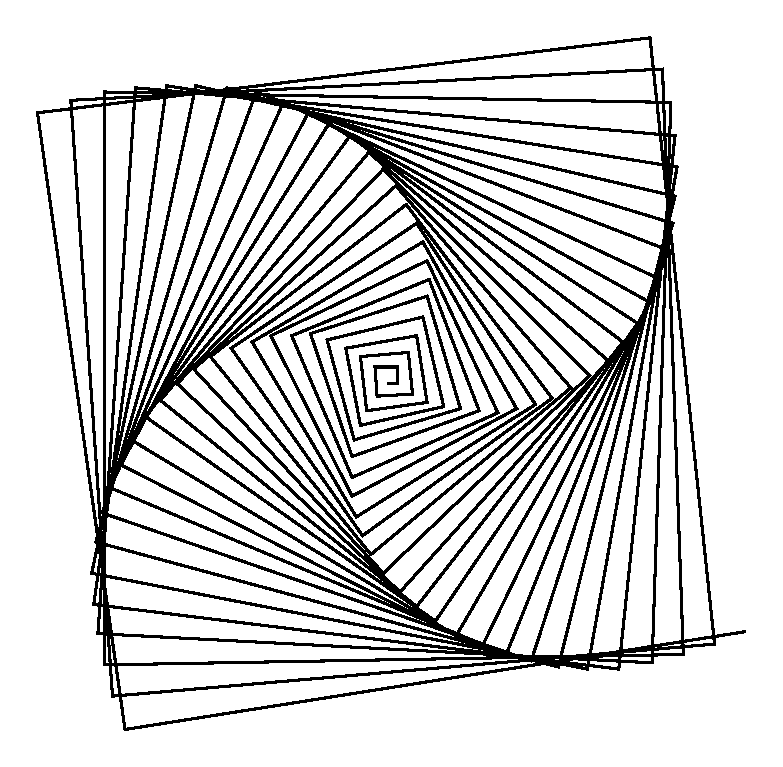
\includegraphics[width=0.9\linewidth]{varLoopsTitle}
\end{chapterfigure}


\hidden{
this is not the title
\begin{alltt}
| caro length angle |
caro := Bot new.
length := 5.
angle := 179.
200 timesRepeat: [ caro go: length.
                 caro turnLeft: angle.
                 length := length + 5]

the one for the picture
| caro length angle |
caro := Bot new.
length := 5.
angle := 178.
110 timesRepeat: [ caro go: length.
                 caro turnLeft: angle.
                 length := length + 3]
\end{alltt}}


In this chapter we show how to use variables and loops together. We start by analyzing a simple problem that shows the need for using variables with loops. Then you shall experiment with some other problems. 

%We introduce the new messages
%\ct{to:do:} and \ct{to:do:by:} that are more adapted to situations
%where sequences of numbers are needed.

\section{A Motivating Example}

Try to generate the odd stairway shown in Figure~\ref{fig:strangestair}. One way to start would be by generating a normal stairway and modifying it. One of the problems  that you should be facing and need to solve is that the length of each step is constantly growing.

\begin{figure}[!htbp]
\centerline{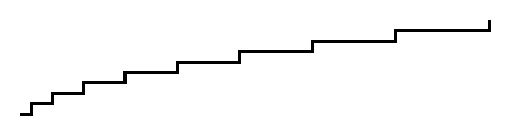
\includegraphics[width=12cm]{varLoopsFlatStair}}
\caption{A strange stair}
\label{fig:strangestair}
\end{figure}

One of the simplest solutions is shown in \scriptref{src:strange1}, where the length of each step grows by 10 pixels. However, such a solution is not satisfactory because we have to compute  the length of the next each step manually. And also because we have to stupidly repeat the same sequence of messages.

\begin{scriptwithtitle}{Strange stair}\label{src:strange1}
| \caro |
\caro := Bot new.
\caro go: \bold{10}.
\caro turnLeft: 90.
\caro go: 5. 
\caro turnRight: 90.
\caro go: \bold{20}.
\caro turnLeft: 90.
\caro go: 5. 
\caro turnRight: 90.
\caro go: \bold{30}.
\caro turnLeft: 90.
\caro go: 5. 
\caro turnRight: 90.
\caro go: \bold{40}.
\caro turnLeft: 90.
\caro go: 5. 
\caro turnRight: 90.
...
\end{scriptwithtitle}

We would like to be able to use the power of variables combind with the power of loops. First you can avoid repeating  the sequence of messages by using the \timesRepeat method.  Second if we study \scriptref{src:strange1}, we see that the length of a step is the length of the previous step plus 10 pixels. Here, like this: 20 = 10 + 10, 30 = 20 + 10, 40 = 30 + 10, and so on as shown by Figure~\ref{fig:stairExplained}.

\begin{figure}[h]
\begin{center}
\includegraphics{stairExplained}
\end{center}
\caption{The length of a step is the length of the previous step plus 10 pixels.}\label{fig:stairExplained}
\end{figure}

If we use the variable \ct{length} to represent the length of a step, the length of the second step is the length of the first step plus 10, and the length of the third step is the length of the second step plus 10... and likewise for the other steps. We can express this by the expression \ct{length\ :=\ length\ + 10} which increases the value of the variable \ct{length} by 10.

Let's combine everything! Now if we take the script of a normal stairway (\scriptref{src:normalstair}), introduce the variable \ct{length} we obtain the same stairway
(\scriptref{src:normalstairlength}).  Then if we add the line \ct{length := length + 10} to change the \ct{length} value in each step of the loop, we get`` the stairway we want (\scriptref{src:strangestair}).

\begin{scriptwithtitle}{A stairway with normal steps}\label{src:normalstair}
| \caro |
\caro := Bot new.
10 timesRepeat: 
               [ \caro go: 10.
               \caro turnLeft: 90.
               \caro go: 5.
               \caro turnRight: 90 ]
\end{scriptwithtitle}

\begin{scriptwithtitle}{A stairway with normal steps using \ct{length}}\label{src:normalstairlength}
| \caro \bold{length}|
\caro := Bot new.
\bold{length := 10.}
10 timesRepeat: 
               [ \caro go: \bold{length.}
               \caro turnLeft: 90.
               \caro go: 5.
               \caro turnRight: 90 ]
\end{scriptwithtitle}

\begin{scriptwithtitle}{The Solution}\label{src:strangestair}
| \caro \bold{length} |
\caro := Bot new.
\bold{length := 10.}
10 timesRepeat: 
               [ \caro go: \bold{length}.
               \caro turnLeft: 90.
               \caro go: 5.
               \caro turnRight: 90.
               \bold{length := length + 10} ]
\end{scriptwithtitle}


In   \scriptref{src:strangestair}, the sequence of messages in the loop first makes the robot go forward a distance given by the value of the variable \ct{length} (10 the first time). Then the robot turns, draws the riser (straight up) and turns again.  Then the value of the variable \ct{length} is increased by 10 and the loop restarts  but with the variable \ct{length} having the new larger value (20 for the second repetition). The whole process is repeated 10 times.

You can't leave out the expression \ct{length\ :=\ length + 10} otherwise the value of the variable will never change.

\begin{exonofig}
Try changing the last line of the loop --- for example put \ct{length\ :=\
length\ +\ 15}.  Then try moving the line to different places in the
loop. Can you explain what happens when you move the last line of the
loop to the beginning of the loop?
\end{exonofig}


If you need more time to understand \scriptref{src:strangestair}, we suggest you think carefully about the value of the variable  \ct{length}, especially at the beginning and end of the loop. Figure out what value \ct{length} has in each message for three repetitions of the loop. If necessary read Chapter~\ref{ch:variables} again.

\section{Practicing: Mazes, Spirals and More}

Let's see how combining variables and loops helps us  solve
some other problems.

\begin{exofig}{varLoopsSquareStair}
Change \scriptref{src:strangestair} to produce the picture shown on the right.
\end{exofig}


\begin{exofigwithsizeandtitle}[0.4]{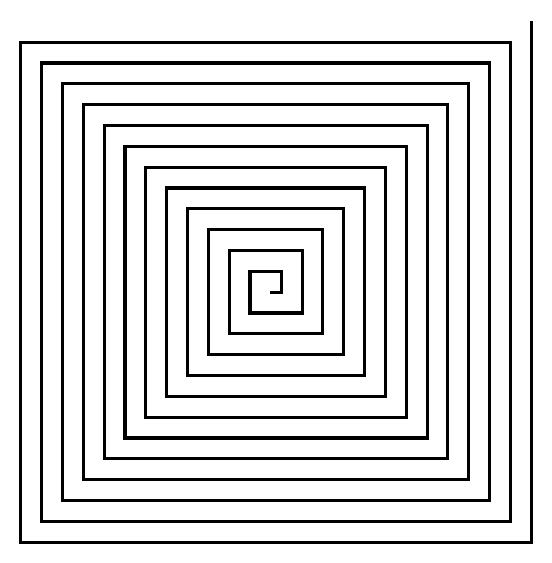
\includegraphics[width=6cm]{varLoopsMaze}}{Maze}\label{exo:maze}
Define a script that reproduces the drawing shown on the right. In addition, by turning through different angles you should be able to recreate the picture at the beginning of the chapter, as well as the spiral shown in  Figure~\ref{fig:spiral}.
\end{exofigwithsizeandtitle}

\begin{figure}
\begin{center}
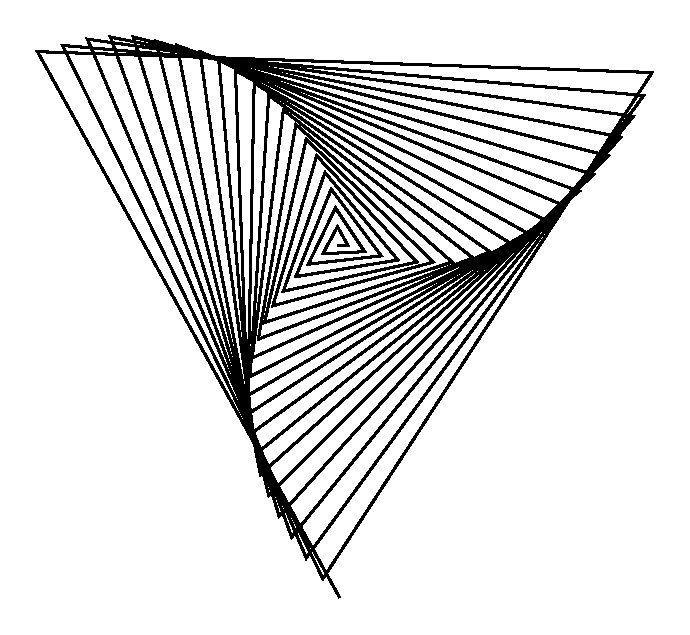
\includegraphics[width=8cm]{varLoopsSpiral121}
\caption{A nice spiral\label{fig:spiral}}
\end{center}
\end{figure}

\begin{exofigwithsizeandtitle}[0.5]{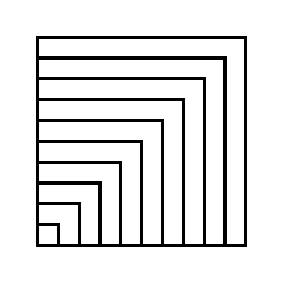
\includegraphics[width=6cm]{Argmirescr}}{Russian squares}\label{exo:russianSquaressimple}
Build the squares of different sizes as shown on the right. Start for example by defining a loops drawing 10 times the same square, then introduce a variable representing the size of the square and finally make it grows over time.
\end{exofigwithsizeandtitle}


\begin{exofigwithsizeandtitle}[0.5]{\includegraphics[width=6cm]{corridor}}{Corridor}\label{exo:corridorsimple}
Build the squares of different size shown on figure on the right.
Again start by drawing a square but draw it starting from its center so that changing its size will automatically draw another square centered around the first one. Then define the square inside a loop, then introduce a variable representing the size of the square and finally make it grows over time.
\end{exofigwithsizeandtitle}



\section{Some Important Points}
Now that you saw the overall process and experimented, we want to stress some 
important points. Script~\ref{src:sketch} shows a skeleton of a typical situation: (1) first a variable is declared, then (2)  it is initialized. After inside the loop the variable is used to perform some computations and (4) its value is changed. 

\begin{scriptwithtitle}{Skeleton of using a variable in a loop}\label{src:sketch}
| \textbf{length} pica |                                      "variable declaration"
...
\bold{length := 10.}                                       "initialization of the variable"
...
10 timesRepeat: 
               [ \caro go: \bold{length}.                  "variable use"
               ....
               \bold{length := length + 10} ]        "variable change of value"
\end{scriptwithtitle}


\paragraph{Variable Initialization.} When you introduce a variable in a loop, you have to pay attention to the first value of the variable, that is, when it is initialized. Normally variable initialization should outside of the loop, else the variable value would be always reinitialized at each loop step and the variable value would not change its value. 


\paragraph{Variable Value Use and Change.} Inside the loop the variable value is often used to perform other computations such as computing other variable values. Then it eventually gets its value changed. In the stairway example, the expression \ct{length := length + 10} increases the value of length based on its preceding value. What is important to understand is that the new change value will be the variable value for the next step of the loop as illustrated by Figure~\ref{fig:steppingLoop}.

\begin{figure}[h]
\begin{center}
\includegraphics[width=12cm]{steppingLoop}
\end{center}
\caption{The length of a step is the length of the previous step plus 10 pixels.
The last value of a variable in the loop body is the variable value for the next step.}
\label{fig:steppingLoop}
\end{figure}



\section{Advanced Experiments}

\begin{exofigwithsizeandtitle}[0.35]{\includegraphics[width=5cm]{damier}}{Squares}\label{exo:spiralsimple}
Define a script that creates the construction shown on the right. This experiment is a bit more complicated than the earlier experiments. Several solutions are possible but to help you we propose some hints: For example start draw a line composed of a certain number of squares, then define a loop that draws this line several times, finally introduce another loop that draws several lines. 
\end{exofigwithsizeandtitle}

\begin{exofigwithsizeandtitle}[0.35]{\includegraphics[width=4cm]{cubesandpyramid}}{Pyramid}\label{exo:spiralsimple}
Define a script that creates the construction shown on the right. This experiment is  a bit more complicated than the earlier experiments.  There are several different scripts that will work. Hints: in the solution of the previous experiment introduce a variable representing the number of lines and change it at each step of the loop. 
\end{exofigwithsizeandtitle}



\summa

\begin{itemize}
\item When introducing a variable inside a loop, be careful about the first value of the variable, that is how the variable is initialized. Normally the initialization occurs outside the loop else the value would always stay the same. 
\item Pay attention that the last value change of a variable in a loop body is the variable value of the next loop step.
\end{itemize}

\ifx\wholebook\relax\else
\end{document}\fi
